\nsecbegin{Ziel des Sprints}
Ziel des Sprints ist, einen möglichst funktionalen Zwischenstand zu erreichen, der die Spezifikation erfüllt. Insbesondere Unit-Tests für die einzelnen Teile sowie die Weiterentwicklung der Sequenzdiagramm-Generierung sollen implementiert werden.

% HIER NEUES KLASSENDIAGRAMM HINZUFUEGEN
%\begin{figure}[hbtp]
%\centering
%\includegraphics[scale=0.5]{}
%\caption{Klassendiagramm des Sprints}
%\end{figure}
\nsecend

\nsecbegin{User-Stories des Sprint-Backlogs}
\nsecbegin{Sequenzdiagramme}
\nsecbegin{Auswahl des zu erstellenden Diagramms}
Als Benutzer wünsche ich mir, dass eine Auswahl zwischen Klassen- und Sequenzdiagrammen möglich ist, damit ich diese je nach meinen Bedürfnissen generieren kann.
\nsecend

\nsecbegin{Generierung von Sequenzdiagrammen}
Als Benutzer wünsche ich mir, Sequenzdiagramme erstellen zu können, um einen Überblick über die Abläufe meines Programms zu erhalten.
\nsecend
\nsecend%Sequenzdiagramme
\nsecend % {User-Stories des Sprint-Backlogs}

\nsecbegin{Zeitliche Planung}
\begin{figure}[hbtp]
\centering
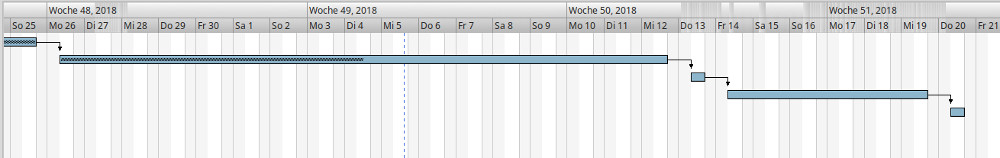
\includegraphics[width=\textwidth]{Bilder/gantt}
\caption{Gantt-Diagramm für Sprint 1}
\end{figure}
\nsecend%Zeitliche Planung

\nsecbegin{Liste der durchgeführten Meetings}
\begin{itemize}
\item Planning-Meeting (29.04.2019)
\item Zwischenstandspräsentation (06.05.2019)
\item Review-Meeting (10.5.2019)
\end{itemize}
\nsecend%Liste der durchgeführten Meetings

\nsecbegin{Ergebnisse des Planning-Meetings}
Die XML- und Textspezifikationen und deren Transformationen sind allen Teams bekannt. Die Grundlage für die Weiterentwicklung der Sequenzdiagramm-Generierung ist damit gelegt. 
\nsecend

\nsecbegin{Aufgewendete Arbeitszeit pro Person$+$Arbeitspaket}
\begin{longtable}{|p{4cm}|l|l|l|l|l|}
        \hline
        Unit-Tests für den Gesamtaufruf & Johann Gerhardt & 01.05.19 & 13.05.19 & 8 &\\
        \hline
        Neue Rahmenstruktur erstellen & Marian Geißler & 29.04.19 & 01.05.19 & 5.5 &\\ \hline
        GUI zu AWT/SWING umbauen & Julian Uebe & 29.04.19 & 13.05.19 &  & \\ 
		\hline
        Generator für Sequenzdiagramme & Elisabeth Schuster & 29.04.19 & 01.05.19 & 8.5 & SequenzDiagramGenerator.java\\
        \hline
        Generator für Sequenzdiagramme & Leo Rauschke & 29.04.19 & 01.05.19 & 13 & SequenzDiagramGenerator.java\\
        \hline
        Ausgabe für Sequenz- und Klassendiagramme & Tore Arndt & 07.05.19 & 13.05.19 & 20 &\\
        \hline
        Generator für Klassendiagramme & Marian Geißler & 29.04.19 & 13.05.19 & 3.5 &\\
        \hline
        Generator für Klassendiagramme & Johann Gerhardt & 01.05.19 & 13.05.19 & 16 &\\
        \hline
        Parser umbauen & Michael Lux & 08.05.19 & 13.05.19 & 14 &\\
        \hline
        Parser umbauen & Jona Meyer & 08.05.19 & 13.05.19 & 10 &\\
        \hline
        \\
        \hline
        \\
        \hline
        \\
\hline
\end{longtable}     
\nsecend

\nsecbegin{Konkrete Code-Qualität im Sprint}
Aufgrund der Umstrukturierung sind einige Funktionalitäten noch nicht gegeben. Das Durchlaufen der XML-Bäume sollte teilweise noch angepasst werden. Hierfür bietet sich die Verwendung von XPath-Ausdrücken an.
\nsecend%Konkrete Code-Qualität im Sprint

\nsecbegin{Konkrete Test-Überdeckung im Sprint}
Es fehlen noch einige Unit-Tests.
\nsecend%Konkrete Test-Überdeckung im Sprint

\nsecbegin{Ergebnisse des Reviews}
\begin{table}[H]

\begin{tabularx}{\textwidth}{ |l|l|X| }
\hline
\textbf{Klasse} & \textbf{Methode} & \textbf{Anmerkungen}\\
 \hline
%Console & showConsole & Pfad anpassen \\
\hline
\end{tabularx}
\end{table}

Sonstiges:
\begin{itemize}
\item XPath nutzen
\item Rekursive Implementierung beim Abarbeiten von verschachtelten Elementen
\item Fehlende Unit-Tests nachholen
\item Evtl. in späterem Sprint: Handling von Methoden in Bedingungen
\end{itemize}
\nsecend%Ergebnisse des Reviews

\nsecbegin{Abschließende Einschätzung des Product-Owners}

\nsecend%Abschließende Einschätzung des Product-Owners

\nsecbegin{Abschließende Einschätzung des Software-Architekten}
XXX
\nsecend%Abschließende Einschätzung des Software-Architekten

\nsecbegin{Abschließende Einschätzung des Team-Managers}

\nsecend%Abschließende Einschätzung des Team-Managers